\chapter{Neural Networks Introduction}
\section{Neural networks intuition}
\subsection{Neuron and the brain}
neurons is the basic unit of the brain, 
it is a cell that receives electrical and chemical signals from other neurons and processes them.
 The neuron has a cell body, dendrites, and an axon. The cell body contains the nucleus and other organelles.
  The dendrites are the input part of the neuron, they receive signals from other neurons.
 The axon is the output part of the neuron, it sends signals to other neurons.
  The axon is connected to the dendrites of other neurons through synapses. 
  The synapse is the connection between the axon of one neuron and the dendrite of another neuron. 
  The synapse is where the electrical and chemical signals are transmitted from one neuron to another. 
  The brain is made up of billions of neurons that are connected to each other through synapses. 
  The neurons communicate with each other by sending electrical and chemical signals through the synapses. 
  This communication between neurons is what allows the brain to process information and perform complex tasks.

\subsubsection*{Simplified model of a neuron}
A neuron can be modeled as a simple mathematical function that takes an \textbf{input} and produces an \textbf{output}.

\subsection{Demand prediction}
\subsubsection*{Terminology}
\begin{itemize}
    \item \textbf{layer}: a collection of neurons that are connected to each other.
    \item \textbf{input layer}: the first layer of the neural network, it receives the input data.
    \item \textbf{output layer}: the last layer of the neural network, it produces the output data.
    \item \textbf{hidden layer}: a layer that is not the input or output layer.
    \item \textbf{neuron}: a node in the neural network that takes an input and produces an output.
    \item \textbf{activation function}: a function that determines the output of a neuron given its input.
    \item \textbf{activation}: the output of a neuron after applying the activation function. 
    Activstions are higher level features.
\end{itemize}

\begin{notebox}
    \hspace{2em}In the neural network architecture, the input layer receives the input data, the hidden layers process the data, and the output layer produces the output data.
    And the neural networks can have multiple hidden layers, each layer can have multiple neurons, and each neuron can have multiple inputs and outputs.
    It is also called ``multilayer perceptron''. 
\end{notebox}
\noindent
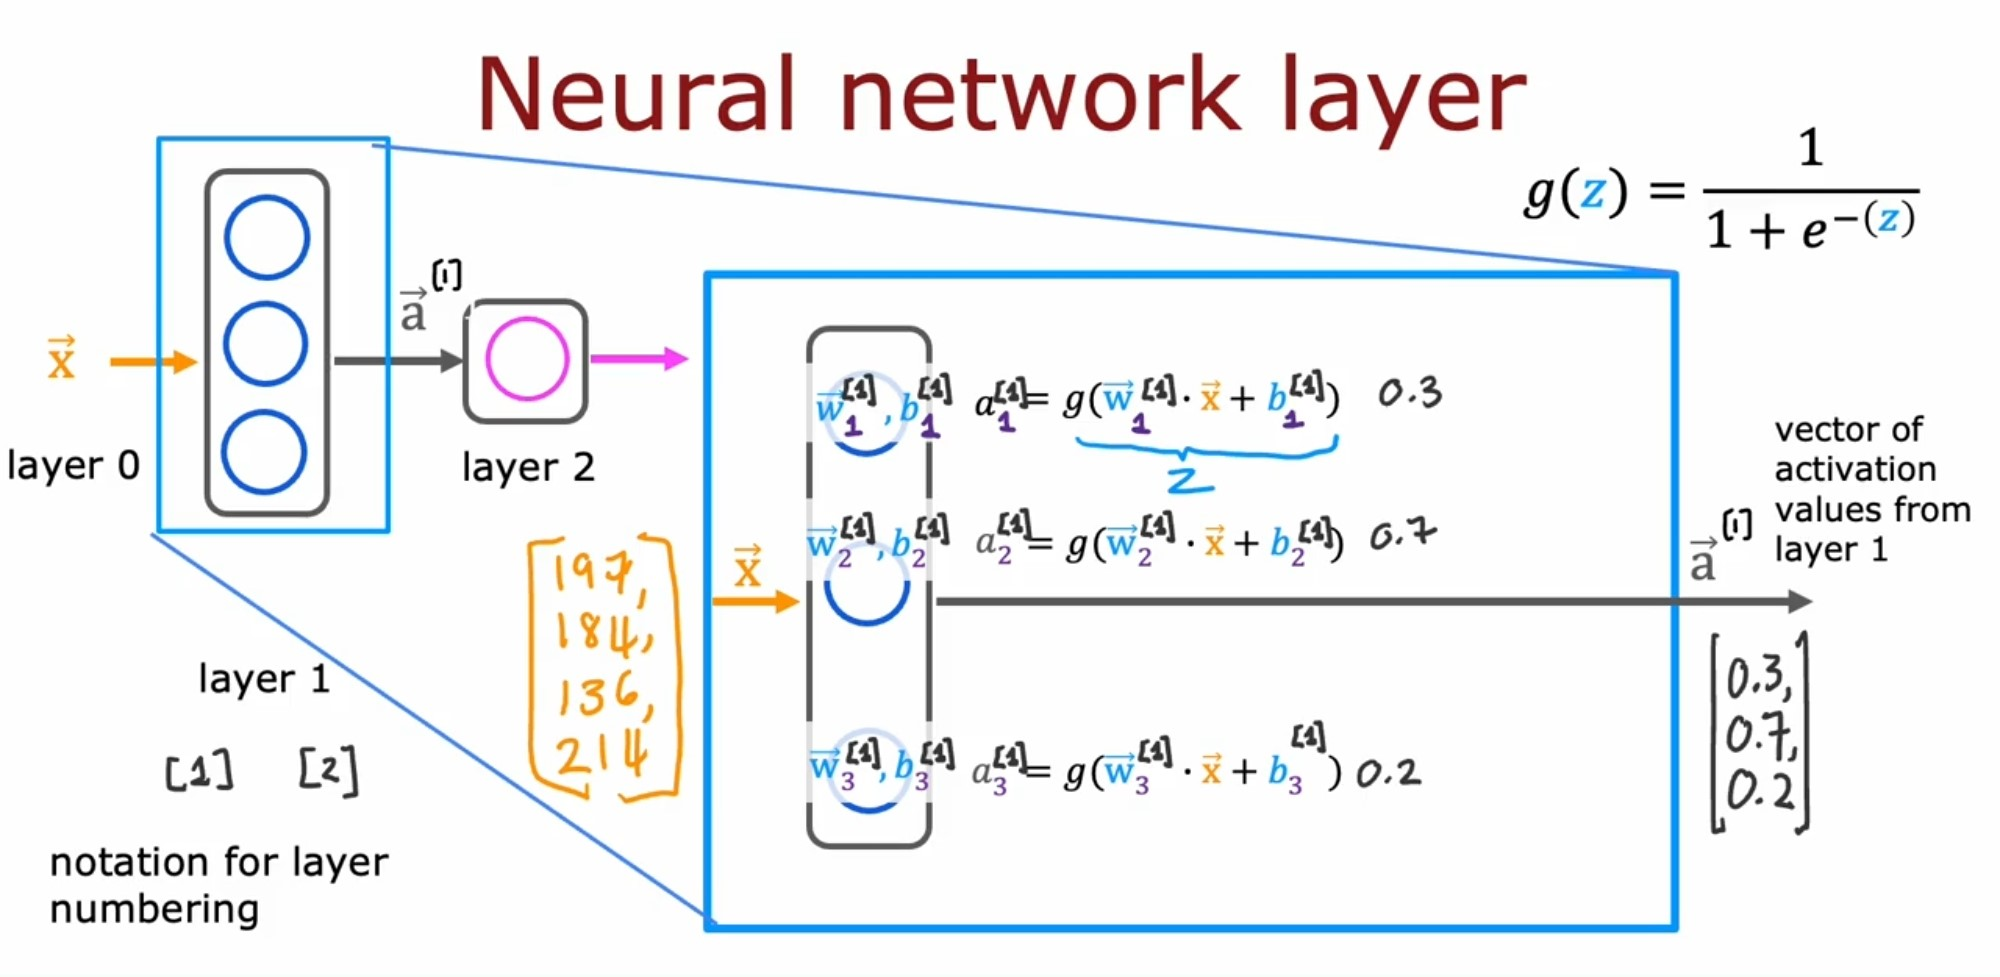
\includegraphics[width=\textwidth]{images/8.1}

\section{Neural networks model}
\begin{notebox}
    \paragraph*{Notation}
    Every layer has a weight matrix $\mathbf{W}$ and a bias vector $\mathbf{b}$.\par
    \hspace{2em}In the layer $j$, the weight matrix $\mathbf{W}^{[j]}$ 
    has the dimension $n^{[j-1]} \times n^{[j]}$ and the bias vector $\mathbf{b}^{[j]}$ has the dimension $1 \times n^{[j]}$.
    Weights of each neuron $\mathbf{w}_i^{[j]}$ are column vectors not scalars. And the input and output vectors $\mathbf{a}$ 
    are both row vectors.
    \begin{equation}
        \mathbf{W}^{[j]} = \begin{bmatrix}
            \mathbf{w}_1^{[j]} & \mathbf{w}_2^{[j]} & \cdots & \mathbf{w}_{n^{[j]}}^{[j]}
        \end{bmatrix}
    \end{equation}
    \begin{equation}
        \mathbf{b}^{[j]} = \begin{bmatrix}
            b_{1}^{[j]}\
            b_{2}^{[j]}\ 
            \cdots\ 
            b_{n}^{[j]}\
        \end{bmatrix}
    \end{equation}
    \hspace{2em}And the layer j takes in the input $\mathbf{a}^{[j-1]}$ and produces the output $\mathbf{a}^{[j]}$ (whose dimension is 
    $n^{[j]}$, the number of neurons of layer j).
    \begin{align}
        a_i^{[j]} &= g(\mathbf{a}^{[j-1]} \cdot \mathbf{w}_i^{[j]} + b_i^{[j]})\\
        (\mathbf{a}^{[j]})^{T} = \begin{bmatrix}
            a_1^{[j]} \\
            a_2^{[j]} \\
            \vdots \\
            a_n^{[j]}
        \end{bmatrix} &=
        \begin{bmatrix}
            g(\mathbf{w}_1^{[j]}\mathbf{a}^{[j-1]} + b_1^{[j]})\\
            g(\mathbf{w}_2^{[j]}\mathbf{a}^{[j-1]} + b_2^{[j]})\\
            \vdots \\
            g(\mathbf{w}_n^{[j]}\mathbf{a}^{[j-1]} + b_n^{[j]})
        \end{bmatrix}
    \end{align}
    \hspace{2em}The dimension of the weight matrix $\mathbf{w}_i^{[j]}$ equals to the previous layer's number
    of neurons $n^{[j - 1]}$, which is the dimension of $\mathbf{a}^{[j - 1]}$.
    $g$ is the activation function such as sigmoid function $g(x) = \frac{1}{1+e^{-x}}$.\par
    \hspace{2em}Taking advantage of the vectorization method, the previous formula can be represented as
    \begin{align}
        \mathbf{a}^{[j]} =  g(\mathbf{a}^{[j - 1]} \cdot \mathbf{W}^{[j]} + \mathbf{b}^{[j]})
    \end{align}
    \hspace{2em} here $\cdot$ is the matrix multiplication, and $g(\mathbf{x})$ means apply $g$ to each element
    in $\mathbf{x}$. 
\end{notebox}
\par
The numbers of neurons in each layer often decrease as we move from the input layer to the output layer.
\par
And the neural network can do inference and predict category.
By looking at the output layer, we can see the probability of each category.
It's a scalar value, if the value is greater than 0.5, then the neural network predicts the certain category.
And this procedure is called \textbf{``forward propagation''}.\par
There are many things neural networks can do, such as image recognition, speech recognition, natural language processing, and many other tasks.\\
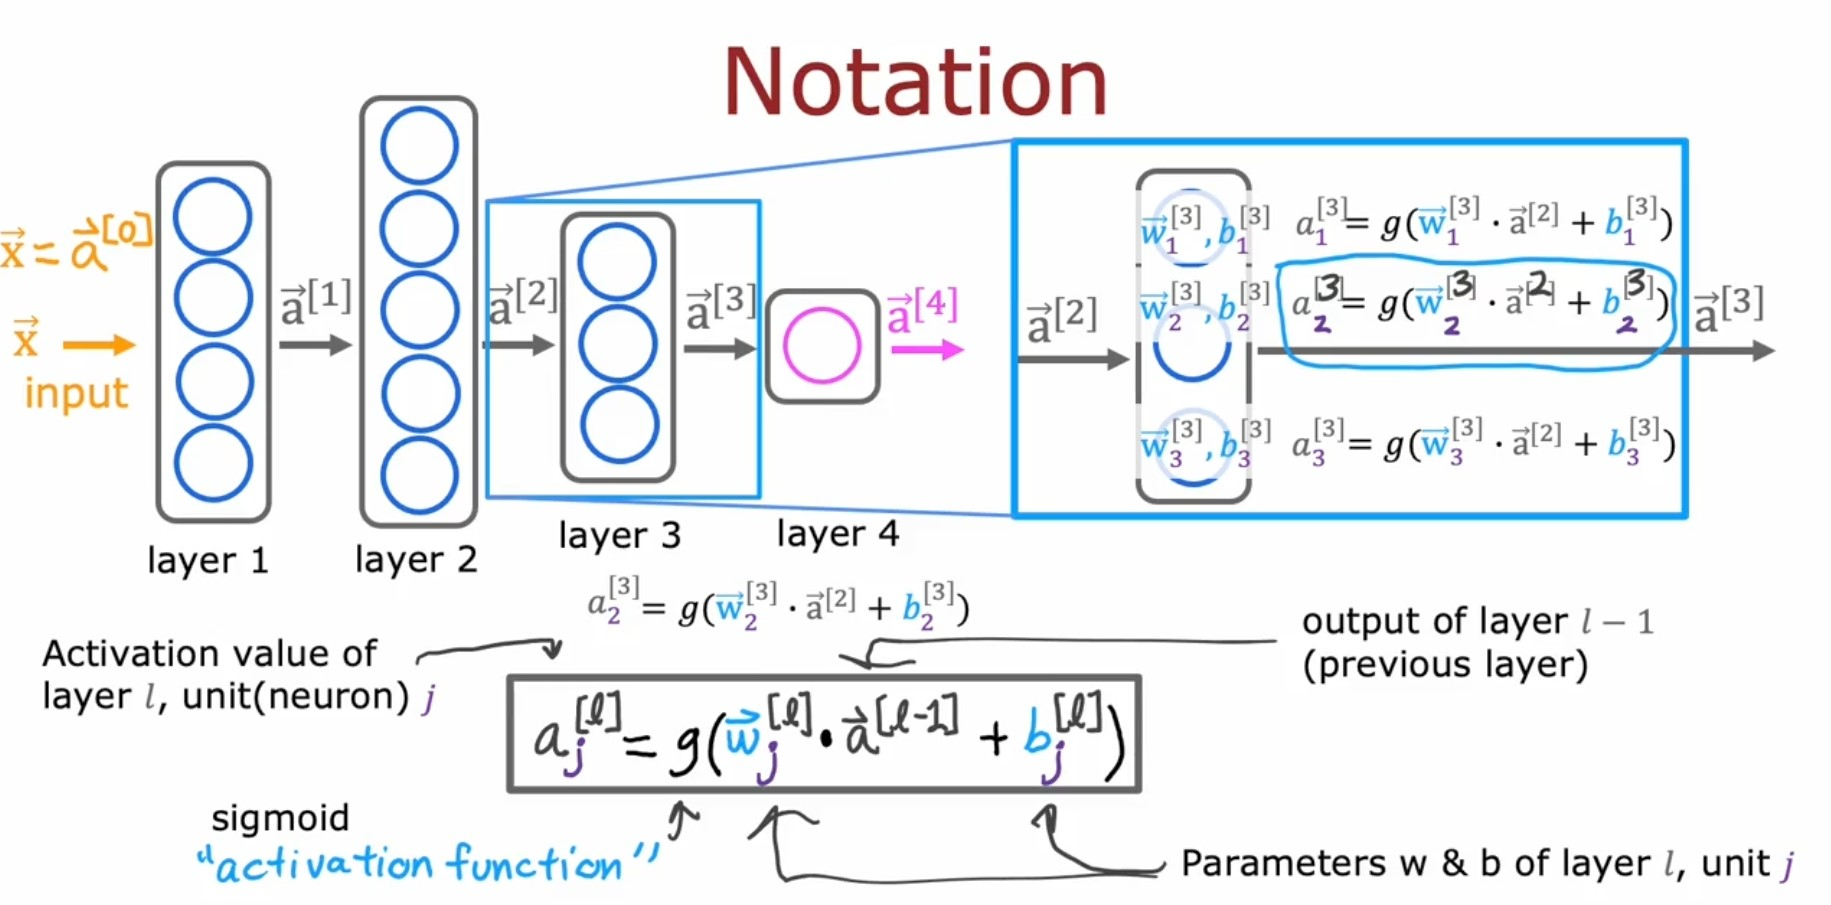
\includegraphics[width=\textwidth]{images/8.2}

\section{Implementation in TensorFlow}
\subsection*{Inference}
Assume you already have a trained model, and you want to use it to make predictions on new data.\par
\begin{center}
    \includegraphics*[width=0.5\textwidth]{images/tf (4)}
\end{center}
\begin{minted}{python}
    x = np.array([[200.0, 17.0]])
    layer_1 = Dense(units=3, activation='sigmoid')
    a1 = layer_1(x)

    layer_2 = Dense(units=1, activation='sigmoid')
    a2 = layer_2(a1)

    if a2 >= 0.5:
        yhat = 1
    else:
        yhat = 0
\end{minted}

\begin{center}
    \includegraphics*[width=0.5\textwidth]{images/tf (1)}
\end{center}
\begin{minted}{python}
    x = np.array([[0.0, 245.0, ..., 240.0, 0.0]])
    layer_1 = Dense(units=25, activation='sigmoid')
    a1 = layer_1(x)

    layer_2 = Dense(units=15, activation='sigmoid')
    a2 = layer_2(a1)

    layer_3 = Dense(units=1, activation='sigmoid')
    a3 = layer_3(a2)

    if a3 >= 0.5:
        yhat = 1
    else:
        yhat = 0
\end{minted}

\subsection*{Data in TensorFlow}
The data in TensorFlow is represented as tensors, which are multi-dimensional arrays.
There is a little difference between the data in TensorFlow and the data in NumPy.
But it is easy to convert the data between TensorFlow and NumPy.
\begin{minted}{python}
    x = np.array([[200.0, 17.0]])
    layer_1 = Dense(units=3, activation='sigmoid')
    a1 = layer_1(x)
    # a1 : tf.Tensor([[0.2, 0.7, 0.3]], shape=(1, 3), dtype=float32)
    # a1.numpy() : array([[0.2, 0.7, 0.3]], dtype=float32)
    layer_2 = Dense(units=1, activation='sigmoid')
    a2 = layer_2(a1)
    # a2 : tf.Tensor([[0.8]], shape=(1, 1), dtype=float32)
    # a2.numpy() : array([[0.8]], dtype=float32)
\end{minted}
\textbf{The example of ``Coffee Roasting'' in optional lab, you may find helpful.}

\section{Building a neural network in TensorFlow}
\textbf{How to build a neural network in TensorFlow?}
\begin{minted}{python}
    model = Sequential([
        Dense(units=3, activation='sigmoid'),
        Dense(units=1, activation='sigmoid')
    ])

    x = np.array([[200.0, 17.0],
                    [100.0, 24.0],
                    [150.0, 20.0],
                    [110.0, 22.0]])
    y = np.array([1, 0, 1, 0])

    model.compile(...)
    model.fit(x, y)

    model.predict(x_new)
\end{minted}

\section{Forward propagation}
\textbf{How to implement forward propagation in python?}
\begin{minted}{python}
    def dense(a_in, W, b):
        units = W.shape[1]
        a_out = np.zeros(units)
        for j in range(units):
            w = W[:, j]
            z = np.dot(w, a_in) + b[j]
            a_out[j] = sigmoid(z)
        return a_out
\end{minted}
\par
\textbf{Dense layer vectorized implementation}
\begin{minted}{python}
    def dense(a_in, W, b):
        z = np.dot(a_in, W) + b
        # z = np.matmul(a_in, W) + b
        a_out = sigmoid(z)
        return a_out
\end{minted}
\par
\textbf{Sequential forward}
\begin{minted}{python}
    def sequential_forward(x, model):
        a = x
        for layer in model:
            a = dense(a, layer['W'], layer['b'])
        return a
\end{minted}
